\section{System's perspective}

\subsection{Design and architecture}

When we first began the project, we opted to use our Chirp! project from the BDSA course. There were multiple reasons for this. Firstly, Helge recommended using Chirp!, and secondly, all group members were already familiar with the codebase, which we believed would make it easier to solve problems, understand each other’s code, and improve maintainability.

We dockerized our application in order to deploy it across multiple servers, as illustrated in Figure \ref{fig:UML-Deployment-Diagram}, which presents a simplified overview of the deployment architecture and therefore does not include every container used within the system. To separate responsibilities within the system, we utilized multiple DigitalOcean droplets dedicated to services such as the web server, API server, database, monitoring infrastructure, and load balancers. By separating the system components, it became easier to deploy, update and monitor without affecting the rest of system.

As shown in Figure \ref{fig:UML-Load-Balance-Diagram}, the system also utilizes load balancing to distribute incoming traffic between multiple application servers. This improves our system's scalability and availability by ensuring that requests can be handled across different server instances instead of relying on a single deployment.

\begin{figure}[H]
    \centering
    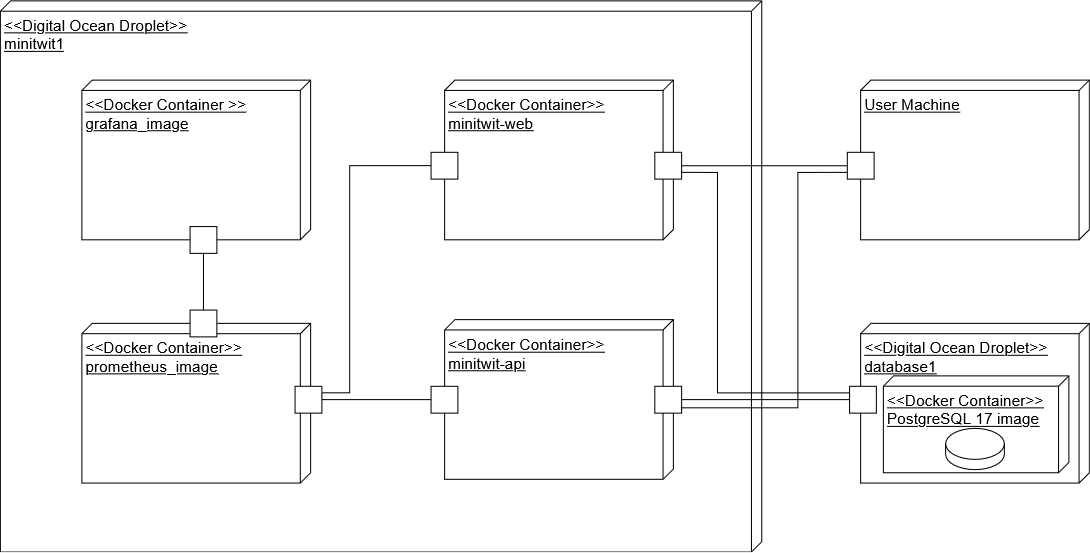
\includegraphics[scale=0.39]{images/DeploymentDiagram.png}
    \caption{MiniTwit Deployment Diagram}
    \label{fig:UML-Deployment-Diagram}
\end{figure}


\begin{figure}[H]
    \centering
    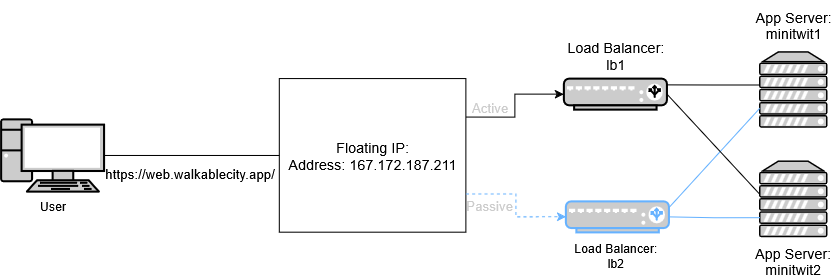
\includegraphics[width=\textwidth]{images/LoadBalancerDiagram.png}
    \caption{MiniTwit Load Balance Deployment Diagram}
    \label{fig:UML-Load-Balance-Diagram}
\end{figure}

\begin{figure}[H]
    \centering
    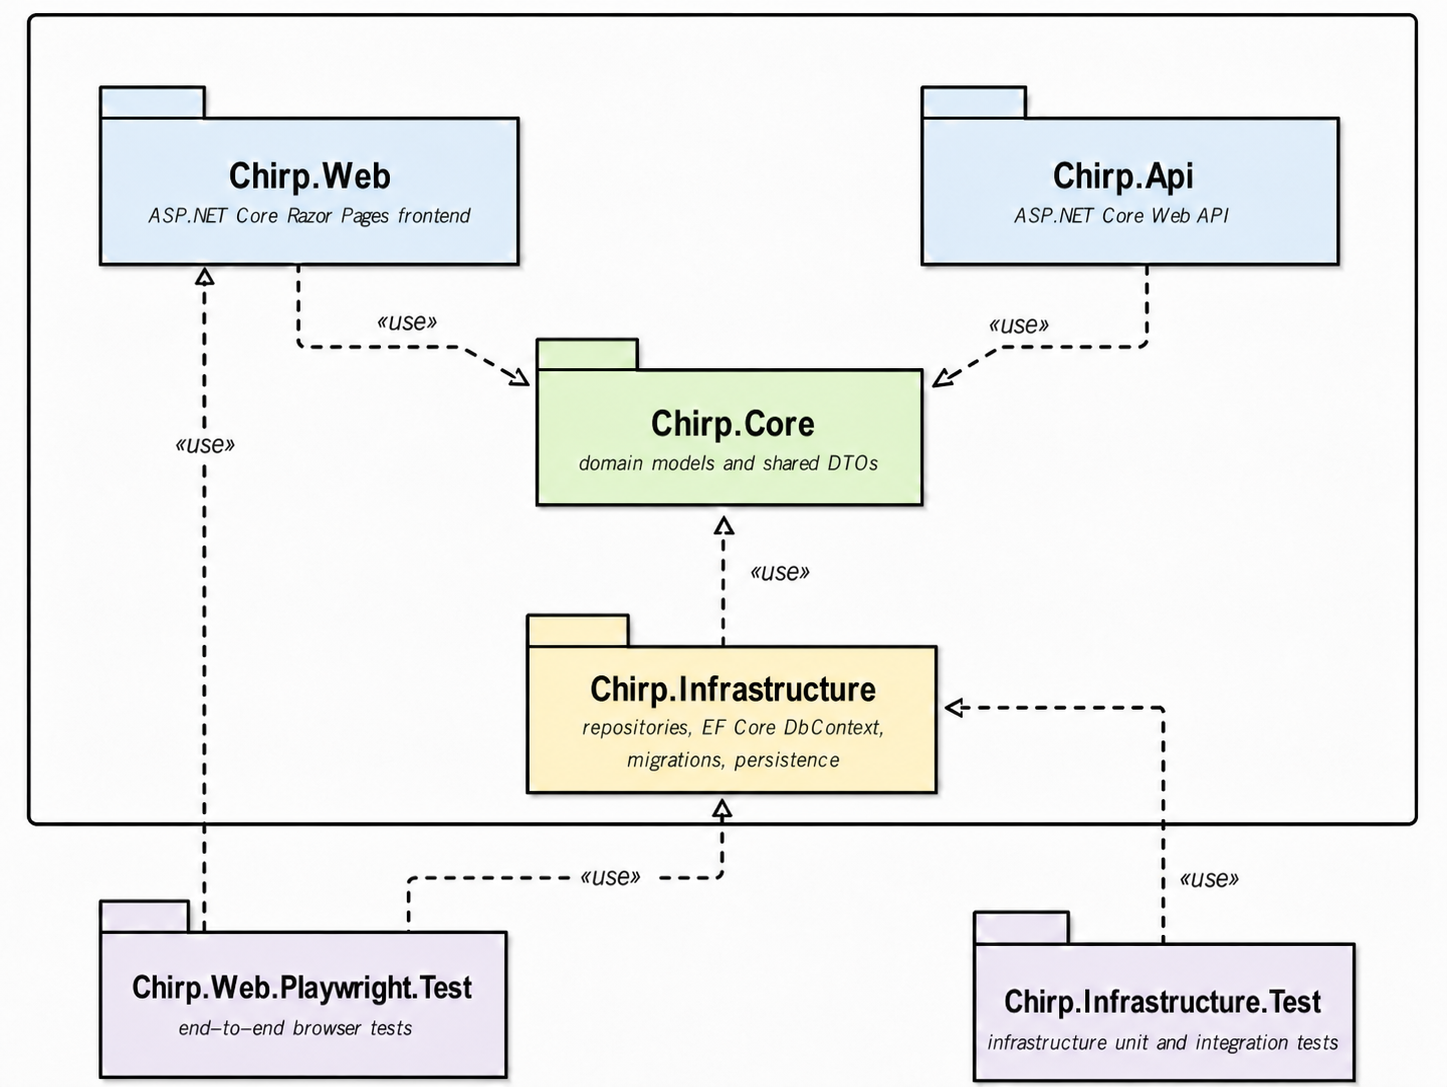
\includegraphics[width=0.8\textwidth]{images/UML-Package-Diagram.png}
    \caption{MiniTwit Package Diagram}
    \label{fig:UML-Package-Diagram}
\end{figure}

\subsection{Dependencies}
The system depends on several technologies and tools across development and operations. 
\begin{itemize}
    \item The main implementation technologies are: C\#, ASP.NET Core, Razor Pages, ASP.NET Identity, EF Core, and PostgreSQL.
    \item Deployment depends on: Docker, Docker Compose, Terraform, Digital Ocean, nginx, and Keepalived.
    \item For operations and observability, the system uses: Prometheus for metrics, Grafana for dashboards, and Loki together with Alloy for centralized logging. 
    \item For quality assurance, the project uses: xUnit, Playwright, Test containers, Coverlet, StyleCop Analyzers, and GitHub Actions.
\end{itemize}

\subsection{Flow}
Below is a sequence diagram, showing the dynamic view and flow of a user posting a message.
It shows the sequence of calls for a message being posted on our application
through the web.

\begin{figure}[H]
    \centering
    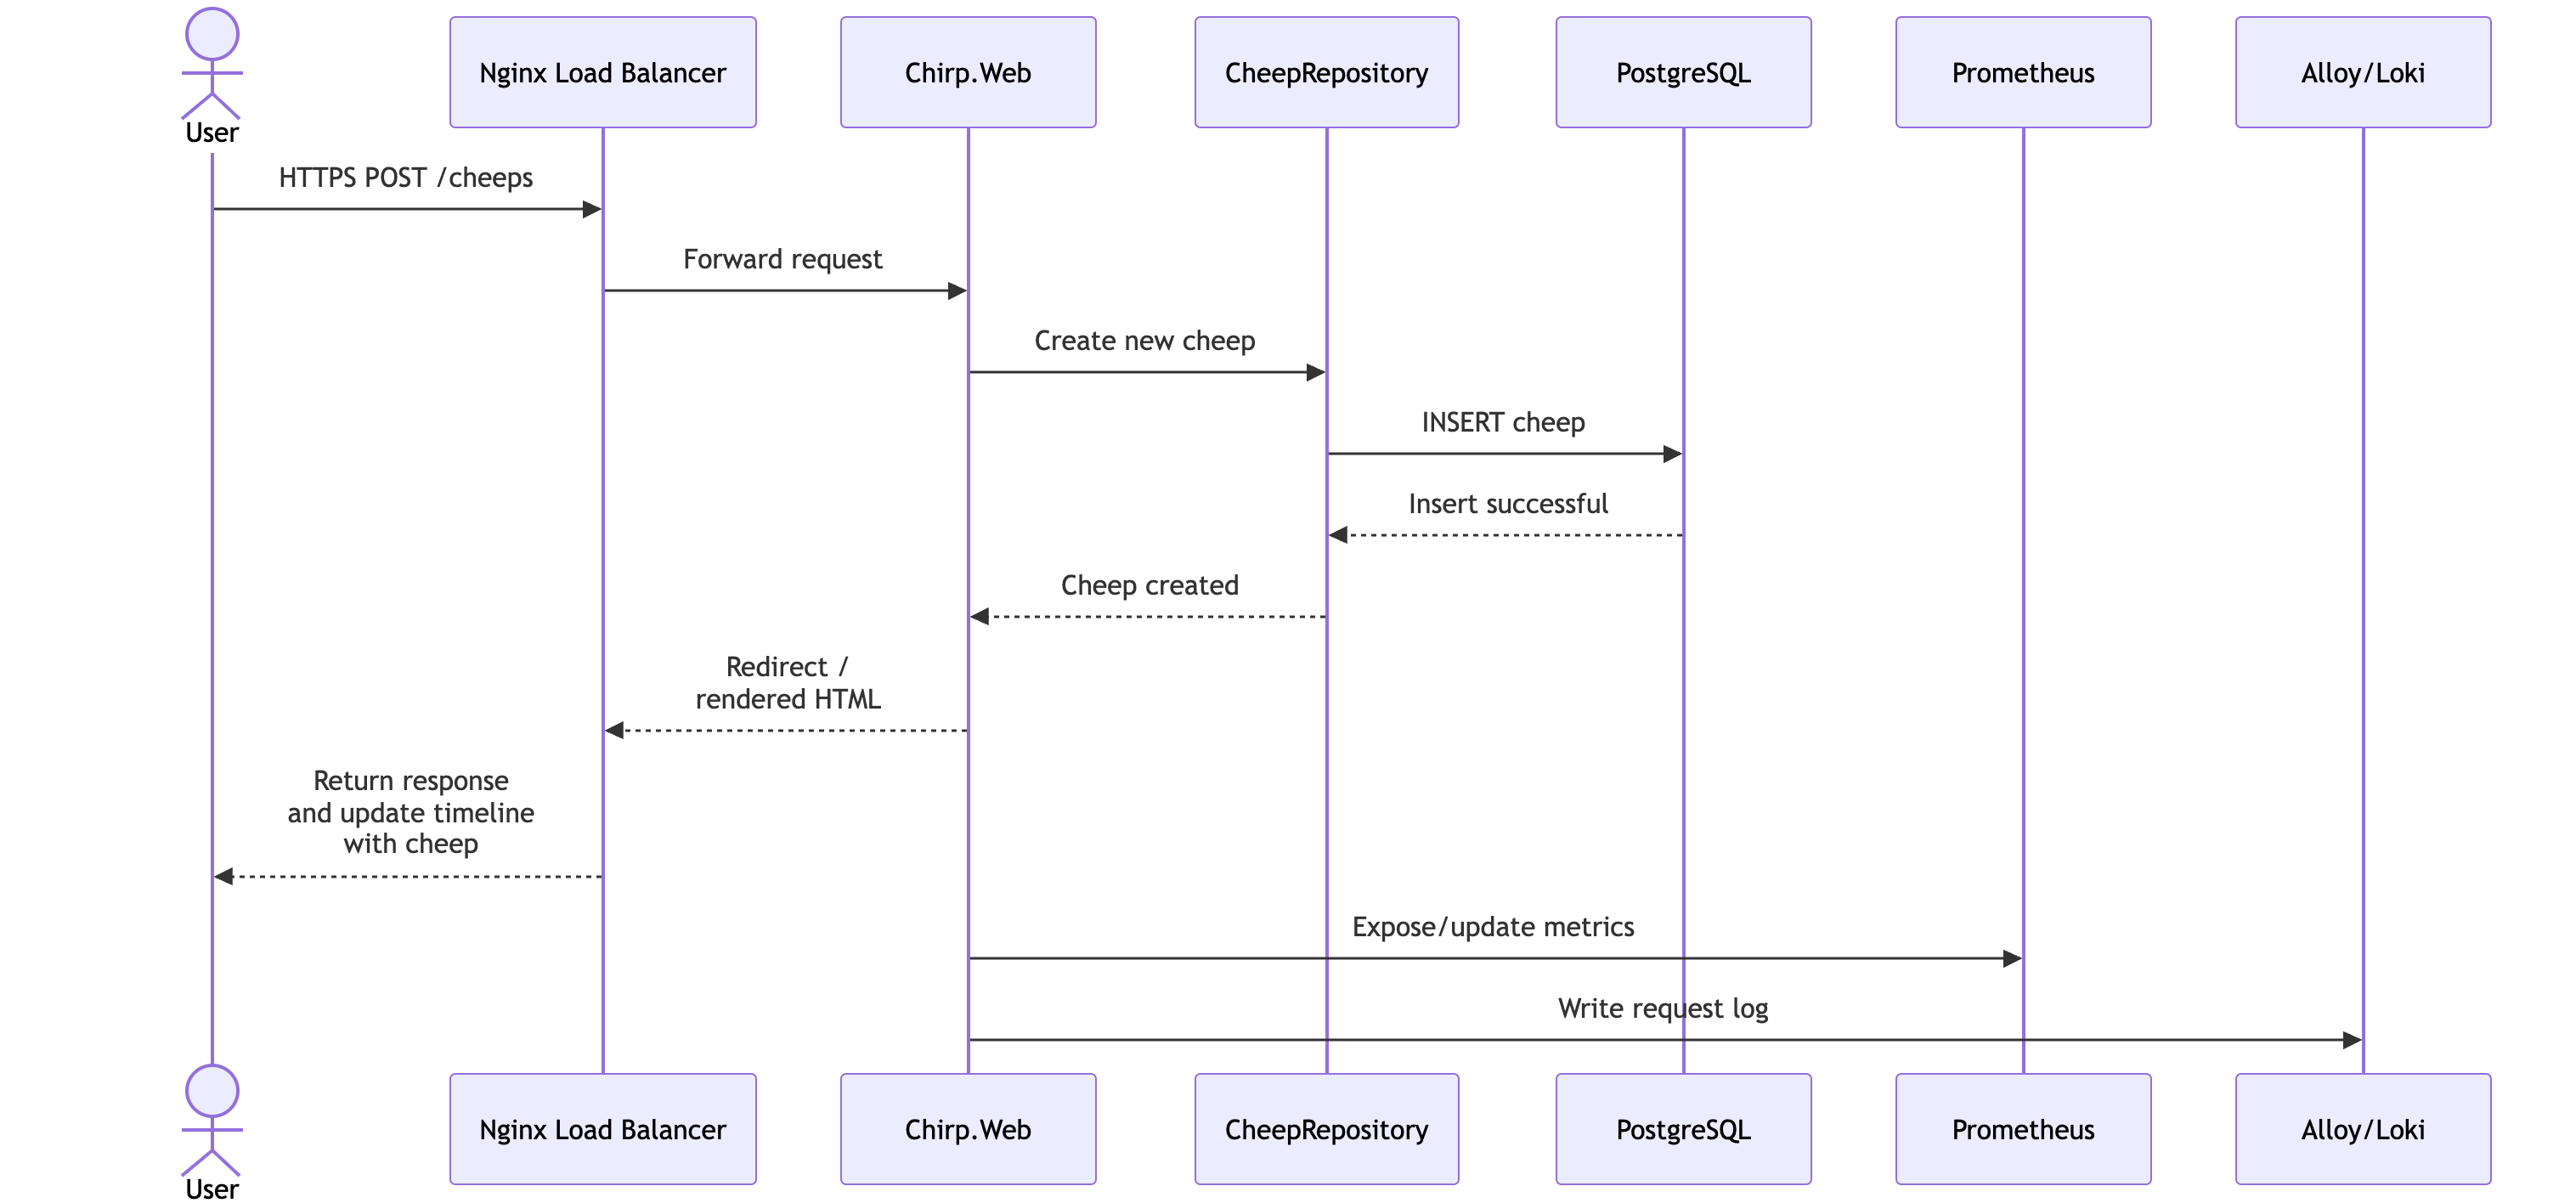
\includegraphics[width=\textwidth]{images/sequence-diagram.png}
    \caption{MiniTwit Sequence Diagram}
    \label{fig:UML-Sequence-Diagram}
\end{figure}

\subsection{Current state}
As shown in Figures \ref{fig:SonarQube-Security} and \ref{fig:SonarQube-Rely-Main}, the reliability, maintainability and security ratings achieved the highest possible score of A. There are however three security hotspots, earning us our lowest score of C. For a more detailed explanation of security within the system, see Section \ref{sec: security}. Furthermore, the code duplication metric is low at 4.2\%, indicating a limited amount of duplicated code. 

\begin{figure}[H]
    \centering
    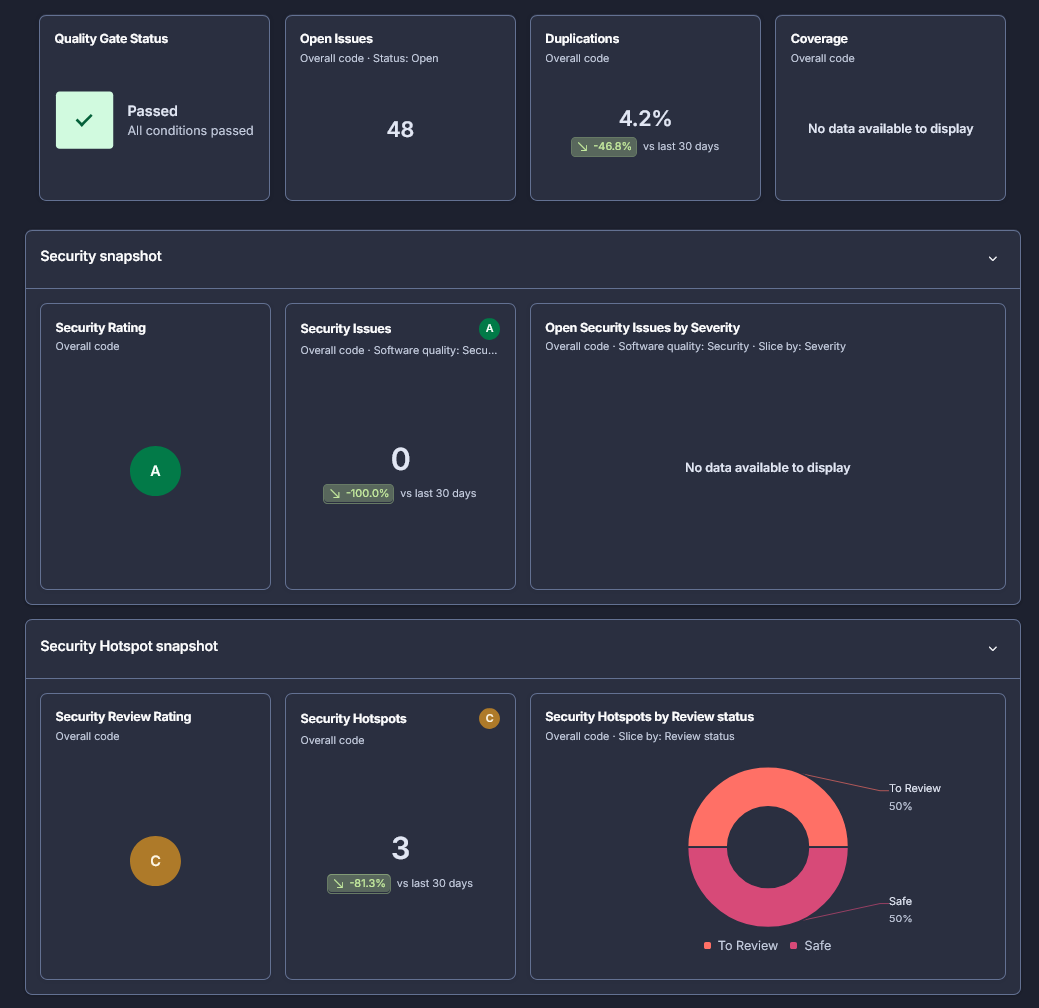
\includegraphics[width=0.8\textwidth]{images/SonarQube-Security.png}
    \caption{SonarQube Security Snapshots}
    \label{fig:SonarQube-Security}
\end{figure}

\begin{figure}[H]
    \centering
    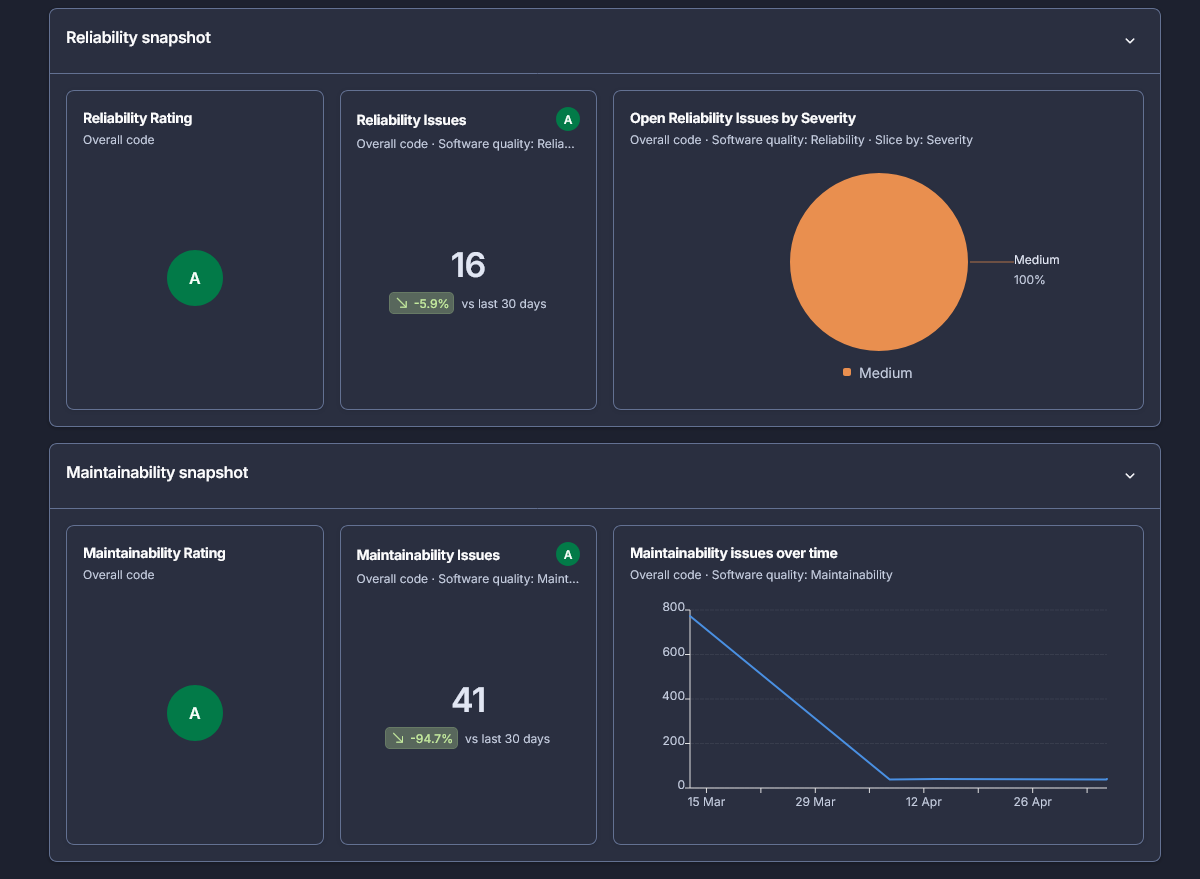
\includegraphics[width=0.8\textwidth]{images/SonarQube-Rely-Main.png}
    \caption{SonarQube Reliability and Maintainability Snapshots}
    \label{fig:SonarQube-Rely-Main}
\end{figure}